%
% tp1.tex
%
% auteurs: Paul Chabanon (PC) et Antoine Guerrée (AG)
% créé le: 2013-06-01
% dernière mise-à-jour: 2013-06-01
%
% Description:
% Fichier principal du document. Contient les commandes LaTeX nécessaires,
% et inclus les autres fichiers nécessaires au rapport.
% Pour compiler ce document, les packages texlive et texlive-lang-french
% texlive-latex-extra sont recommandés.
%


%% En-tête
\documentclass[a4paper,12pt,titlepage]{article}
\usepackage[french]{babel}
\usepackage[utf8]{inputenc} % encodage
\usepackage[T1]{fontenc} % encodage
\usepackage{array} % tableaux
\usepackage[bookmarks=true,colorlinks,linkcolor=blue]{hyperref} % hyperliens
\usepackage{aeguill} % lisibilité
\usepackage{graphicx} % pour insérer des images
\usepackage{amssymb,amsmath} % maths
\usepackage{multicol} % colonnes
\usepackage[francais]{varioref} % chouettes refs
\usepackage{listingsutf8} % to allow utf8 with lstlisting
\usepackage{amsthm} % math proof
\usepackage{float} % mettre les figures où on veut

\lstset{ 
  language=C++,        
  tabsize=3,              
  showstringspaces=false, %pour virer les espaces dans les chaines de caractères
  %basicstyle=\ttfamily\footnotesize,
  %commentstyle=\color{Green}\scriptsize, % white comments
  %keywordstyle=\bfseries,
        %keywordstyle=\color{Blue}\textnormal,
        keywordstyle=\bfseries\ttfamily\color[rgb]{0,0,1},
        identifierstyle=\ttfamily,
        commentstyle=\color[rgb]{0.133,0.545,0.133},
        stringstyle=\ttfamily\color[rgb]{0.627,0.126,0.941},
        showstringspaces=false,
        basicstyle=\small,
        numberstyle=\footnotesize,
  title=\lstname, %afficher le titre
  frame=shadowbox, % le cadre
  captionpos=b, %légende en dessous
  numbers=left, %pour rajouter des numéros de ligne
  stepnumber=5, %définition du pas pour les numéros
  firstnumber=1, %définition du 1er numéro
  breaklines=true,      %pour casser les lignes trop longues
  caption=\lstname,
  inputencoding=utf8/latin1
}


%% Propriétés du document
\title{Compte-rendu de projet IF23\\Système autonome de manipulation de données GPS}
\author{Youenn Piolet \and Julien Nozais \and Alexandre Horréard}
\date{\today} % préférer la date réelle du TP


\begin{document}

\maketitle

\newpage

\section{Présentation du projet}

Le but du projet était de créer le programme tournant sur un micro-contrôleur Arduino permettant de manipuler des données GPS.

Notre boitier récupère les informations envoyées par le module GPS et les stockent sur une carte SD dans des fichiers. 
Ces fichiers peuvent ensuite être récuperés sur un PC pour être utilisés avec GPSprune, un logiciel permettant d'afficher
le parcours correspondant aux données envoyées.

Un premier bouton permet de demarrer ou d'arreter le parcours. Chaque nouveau redemarage créé un nouveau fichier où enregistrer les données.
Chaque parcours est donc enregistré dans un fichier separé. On peut également mettre le parcours sur pause et le redemmarer ensuite, sans changer de parcours.

Le boitier dispose d'un écran LCD qui permet d'afficher plusieurs informations. En appuyant sur un deuxième bouton on change l'affichage.
L'écran peut afficher les coordonnées, la vitesse, la distance parcourue ou l'heure. Toutes ces informations sont bien evidement mises à jour en temps réel.

Un autre bouton permet de choisir le mode d'enregistrement : soit les points sont enregistrés suivant un temps fixe (toutes les trois secondes),
soit les points sont enregistrés suivant leur distance avec le point d'avant. Nous obtenons ainsi une suite de point qui ne sont pas identiques.

L'ensemble fonctionne sur pile. Au demarrage du boitier, la batterie s'affiche sur l'écran LCD.


\section{UML}

\subsection{Diagramme de cas d'utilisation}

\begin{figure}[H]
	\centering
	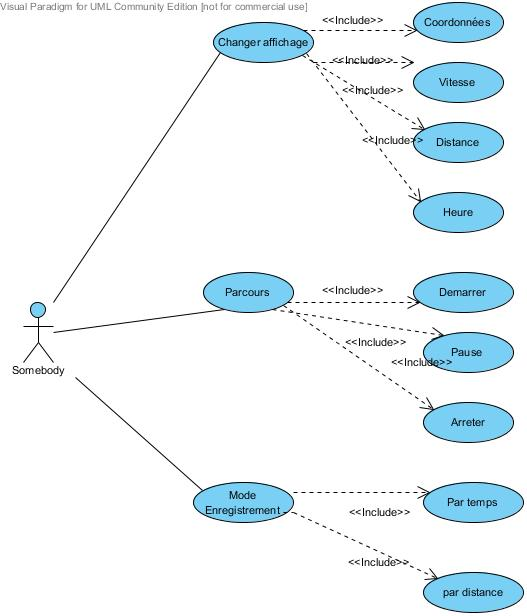
\includegraphics[width=\textwidth]{use_case.jpg}
	\caption{Diagramme de cas d'utilisations}
	\label{usecase}
\end{figure}

\subsection{Diagramme de séquence}

\begin{figure}[H]
	\centering
	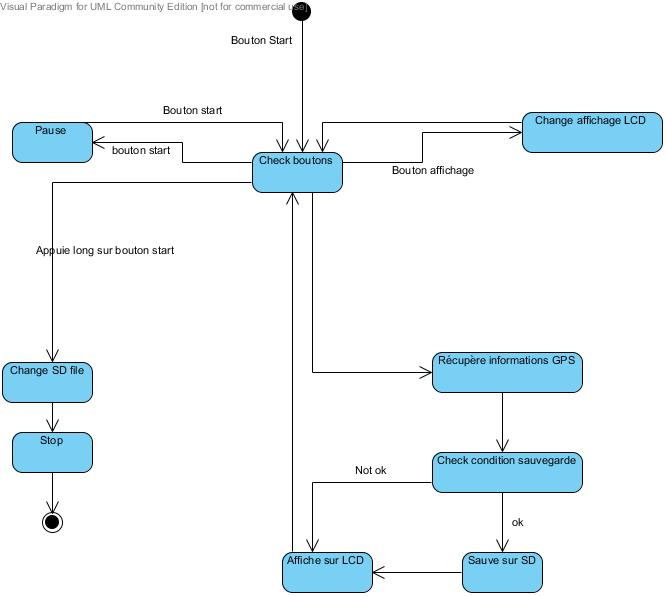
\includegraphics[width=\textwidth]{sequence.jpg}
	\caption{Diagramme de séquence}
	\label{sequence}
\end{figure}

\section{Algorithme}


\end{document}
